% !TEX root = ../main.tex
\section{Measuring Pattern Strength} \label{sec:patternStrength}
  
    \begin{table}[H]
      \begin{tabular}{l || l | l | l | l || l}
        \hline
        {\bf Parameters} & {\bf Shopping} & {\bf Smartphone} & {\bf Bank} & {\bf Training} & {\bf All} \\ \hline
        \#Patterns & 841 & 842 & 838 & 872 & 3393 \\
        Avg. Size & 5.541 & 5.398 & 5.920 & 5.347 & 5.549 \\ 
        Avg. Length & 5.050 & 4.920 & 5.666 & 47886 & 5.103 \\
        \#Intersections & 177 & 149 & 363 & 143 & 832 \\
        Avg. Intersections & 0.210 & 0.1769 & 0.433 & 0.16399 & 0.245 \\
        \#Overlaps & 15 & 12 & 19 & 9 & 55 \\
        Avg. Overlaps & 0.0178 & 0.014 & 0.023 & 0.010 & 0.016\\ \hline
        Avg. Strength & 13.440 & 12.837 & 15.514 & 12.545 & 13.572 \\ 
        Min strength & 6.339 & 6.339 & 6.339 & 6.339 & 6.339 \\
        Max strength & 44.441 & 43.187 & 44.441 & 43.187 & 44.441 \\ \hline
      \end{tabular}
      \caption{Pattern strength}
      \label{tab:patternstrength}
    \end{table}

    {\bf \color{red}{Note-to-self:}}
    \begin{itemize}
      \item Virker som om de fleste mener at banken krever høyest sikkerhetsnivå, men hvorfor ikke bruke det som er sikkert på mer?
      \item Det finnes ikke et eneste passord som oppnår maks styrke på 46.8. Høyeste er 44.3
      \item Gjennomgående er mobil og trening er lavest på alle parametere, mens bank er gjennomsnittlig høyest på alle ledd.
      \item av 3393 mønstre oppstår det bare 55 overlapp, noe som er veldig lavt.
      \item Sjekke hvordan det står til med styrken på topp 20/100 mønstre
      \item Hvordan er styrken basert på alder, kjønn, handedness, finger brukt, etc. 
    \end{itemize}


    \begin{table}[H]
      \centering
      \begin{tabular}{l || l | l || l | l}
        \hline
         & \multicolumn{2}{c ||}{\bf Gender} & \multicolumn{2}{c}{\bf Experience} \\ \hline
        {\bf Parameters}   & {\bf Male} & {\bf Female} & {\bf Yes} & {\bf No} \\ \hline
        \#Patterns         & 2099       & 1102         & 1864      & 1317 \\
        Avg. Size          & 5.673      & 5.309        & 5.667     & 5.368 \\ 
        Avg. Length        & 5.283      & 4.761        & 5.274     & 4.853 \\
        \#Intersections    & 668        & 123          & 572       & 213 \\
        Avg. Intersections & 0.318      & 0.112        & 0.310     & 0.162 \\
        \#Overlaps         & 47         & 6            & 37        & 16 \\
        Avg. Overlaps      & 0.022      & 0.005        & 0.019     & 0.012 \\ \hline
        Avg. Strength      & 14.215     & 12.340       & 14.174    & 12.670 \\ 
        Min strength       & 6.339      & 6.339        & 6.340     & 6.340 \\
        Max strength       & 44.441     & 40.0715      & 44.441    & 44.441 \\ \hline
      \end{tabular}
      \caption{Password strength - Gender and IT/Security experience}
      \label{fig:hello}
    \end{table}


  \begin{figure}[H]
      \centering
      \vspace{1.5cm}
      \subfigure[Sequence: 147852369, \newline Strength: 27.00]{
        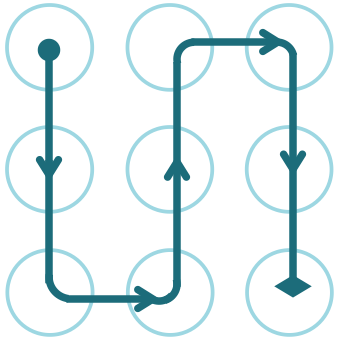
\includegraphics[width=0.27\textwidth]{pics/experiment/strengthpattern2.png}
        \hspace{0.6cm}
      }
      \subfigure[Sequence:213546879, \newline Strength: 36.655]{
        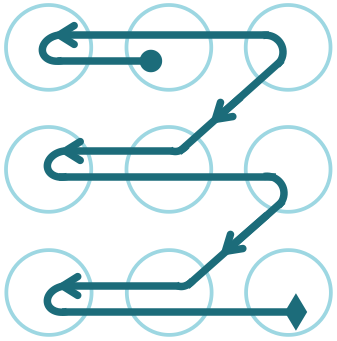
\includegraphics[width=0.27\textwidth]{pics/experiment/strengthpattern3.png}
        \hspace{0.6cm}
      }
      \subfigure[Sequence: 591827346, \newline Strength: 46.807]{
        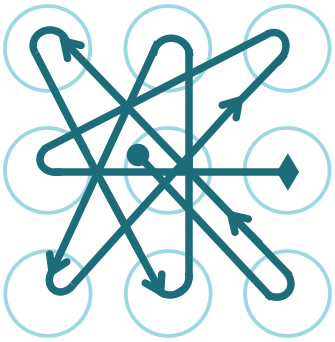
\includegraphics[width=0.27\textwidth]{pics/experiment/strengthpattern1.png}
      }
      \vspace{0.5cm}

      \subfigure[Sequence: 968752, \newline Strength: 15.259]{
        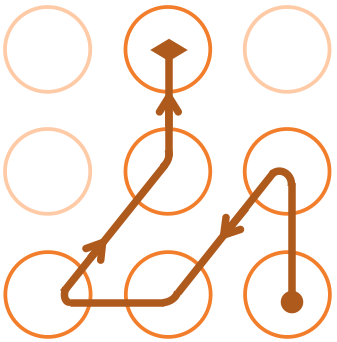
\includegraphics[width=0.27\textwidth]{pics/experiment/strengthpattern7.png}
        \hspace{0.6cm}
      }
      \subfigure[Sequence: 1269853, \newline Strength: 20.781]{
        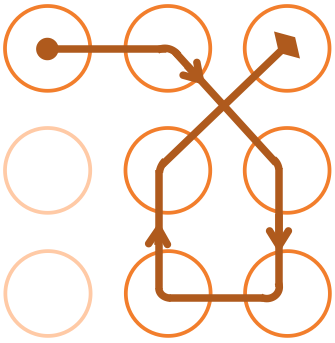
\includegraphics[width=0.27\textwidth]{pics/experiment/strengthpattern8.png}
        \hspace{0.6cm}
      }
      \subfigure[Sequence: 36578249, \newline Strength: 30.512]{
        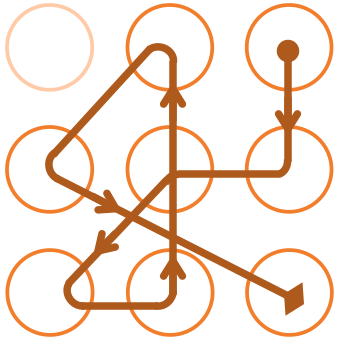
\includegraphics[width=0.27\textwidth]{pics/experiment/strengthpattern9.png}
      }
      
      \vspace{0.5cm}

      \subfigure[Sequence: 1478, \newline Strength: 6.339]{
        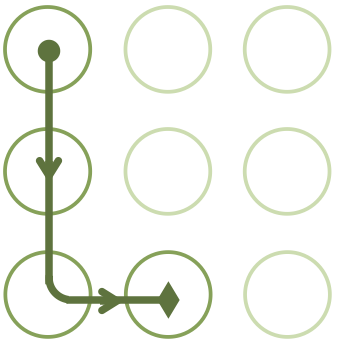
\includegraphics[width=0.27\textwidth]{pics/experiment/strengthpattern4.png}
        \hspace{0.6cm}
      }
      \subfigure[Sequence: 5968, \newline Strength: 9.086]{
        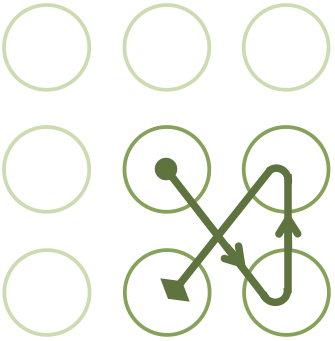
\includegraphics[width=0.27\textwidth]{pics/experiment/strengthpattern5.png}
        \hspace{0.6cm}
      }
      \subfigure[Sequence: 4927, \newline Strength: 11.786]{
        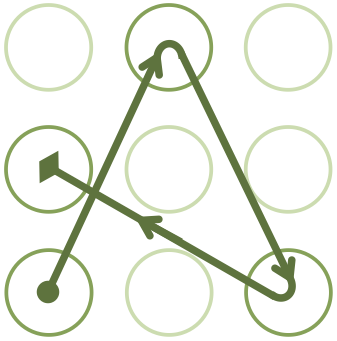
\includegraphics[width=0.27\textwidth]{pics/experiment/strengthpattern6.png}
      }

      \vspace{0.5cm}
      \caption{Examples of patterns with different length and strength}
    \end{figure}


    % \begin{table}[H]
    %   \begin{tabular}{l || l | l}
    %     \hline
    %     {\bf Parameters} & {\bf Male} & {\bf Female} \\ \hline
    %     \#Patterns & &  \\
    %     Avg. Size & & \\ 
    %     Avg. Length & & \\
    %     \#Intersections & & \\
    %     Avg. Intersections & & \\
    %     \#Overlaps & & \\
    %     Avg. Overlaps & & \\ \hline
    %     Avg. Strength & & \\ 
    %     Min strength & & \\
    %     Max strength & & \\ \hline
    %   \end{tabular}
    %   \caption{}
    %   \label{}
    % \end{table}
